\documentclass[aspectratio=169,10pt]{beamer}

% Theme configuration
\usetheme{Madrid}
\usecolortheme{seahorse}

% Custom colors
\definecolor{warmbeige}{RGB}{245, 240, 230}
\definecolor{darkbrown}{RGB}{60, 40, 30}
\definecolor{accentgold}{RGB}{180, 140, 80}
\definecolor{successgreen}{RGB}{80, 140, 80}
\definecolor{alertred}{RGB}{180, 80, 60}

\setbeamercolor{background canvas}{bg=warmbeige}
\setbeamercolor{normal text}{fg=darkbrown}
\setbeamercolor{frametitle}{fg=darkbrown,bg=warmbeige}
\setbeamercolor{title}{fg=darkbrown}
\setbeamercolor{structure}{fg=accentgold}
\setbeamercolor{block title}{fg=white,bg=accentgold}
\setbeamercolor{block body}{fg=darkbrown,bg=white}
\setbeamercolor{item}{fg=accentgold}

% Packages
\usepackage{graphicx}
\usepackage{booktabs}
\usepackage{tikz}
\usetikzlibrary{positioning,shapes,arrows,calc}

% Remove navigation symbols
\setbeamertemplate{navigation symbols}{}

% Title information
\title[GPU Energy Optimization]{\textbf{GPU Energy Optimization for Distributed Training}}
\subtitle{Lock-Frequency Strategy for 20\%+ Power Savings}
\author[Team]{Distributed Training Optimization Team}
\institute[]{Megatron-DeepSpeed Energy Efficiency Project}
\date{\today}

\begin{document}

% Title slide
{
\setbeamertemplate{footline}{}
\begin{frame}
\titlepage
\end{frame}
}

% Agenda
\begin{frame}{Outline}
\tableofcontents
\end{frame}

% Section 1: Background
\section{Background \& Challenges}

\begin{frame}{Energy Challenges in LLM Training}
\begin{columns}
\begin{column}{0.5\textwidth}
\textbf{Industry Pain Points:}
\begin{itemize}
    \item GPT-4 training: \textbf{12M kWh} electricity
    \item Power cost: \textbf{40-60\%} of total cost
    \item Carbon emission constraints
\end{itemize}
\vspace{0.5cm}
\textbf{Limitations of Existing Solutions:}
\begin{itemize}
    \item Dynamic frequency: high complexity
    \item Default config: far from optimal
    \item Lack of accurate prediction tools
\end{itemize}
\end{column}
\begin{column}{0.5\textwidth}
\begin{block}{Our Insight}
\textbf{Static frequency} can achieve significant energy savings without substantially impacting training time.
\end{block}
\vspace{0.3cm}
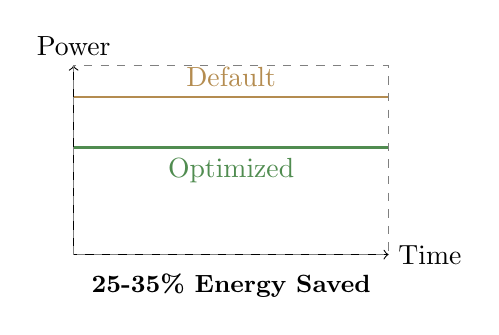
\begin{tikzpicture}[scale=0.8]
    \draw[->] (0,0) -- (5,0) node[right] {Time};
    \draw[->] (0,0) -- (0,3) node[above] {Power};
    \draw[thick,accentgold] (0,2.5) -- (5,2.5) node[midway,above] {Default};
    \draw[thick,successgreen] (0,1.7) -- (5,1.7) node[midway,below] {Optimized};
    \draw[dashed,gray] (0,0) rectangle (5,3);
    \node at (2.5,-0.5) {\small \textbf{25-35\% Energy Saved}};
\end{tikzpicture}
\end{column}
\end{columns}
\end{frame}

\begin{frame}{Core Technical Challenges}
\begin{block}{Central Challenge}
How to find the \textbf{energy-optimal} GPU frequency while \textbf{guaranteeing training efficiency}?
\end{block}
\vspace{0.3cm}
\begin{columns}
\begin{column}{0.33\textwidth}
\centering
\textbf{Challenge 1: Non-linear Frequency-Performance}
\vspace{0.2cm}

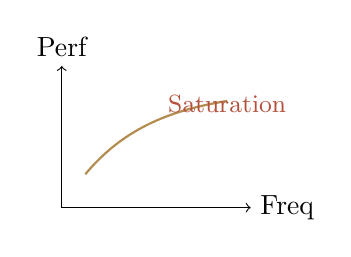
\begin{tikzpicture}[scale=0.6]
    \draw[->] (0,0) -- (4,0) node[right] {Freq};
    \draw[->] (0,0) -- (0,3) node[above] {Perf};
    \draw[thick,accentgold,domain=0.5:3.5,smooth,variable=\x] plot (\x,{2.5*(1-exp(-\x/1.5))});
    \node[alertred] at (3.5,2.2) {\small Saturation};
\end{tikzpicture}

Diminishing returns at high freq
\end{column}
\begin{column}{0.33\textwidth}
\centering
\textbf{Challenge 2: Cross-Node Communication}
\vspace{0.2cm}

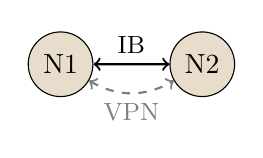
\begin{tikzpicture}[scale=0.6]
    \node[draw,circle,fill=accentgold!30] (n1) at (0,1.5) {N1};
    \node[draw,circle,fill=accentgold!30] (n2) at (3,1.5) {N2};
    \draw[<->,thick] (n1) -- (n2) node[midway,above] {\small IB};
    \draw[<->,thick,dashed,gray] (n1) to[bend right=30] node[midway,below] {\small VPN} (n2);
\end{tikzpicture}

Network-dependent overhead
\end{column}
\begin{column}{0.33\textwidth}
\centering
\textbf{Challenge 3: Topology Diversity}
\vspace{0.2cm}

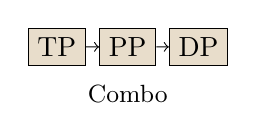
\begin{tikzpicture}[scale=0.6]
    \node[draw,rectangle,fill=accentgold!30] (tp) at (0,2) {TP};
    \node[draw,rectangle,fill=accentgold!30] (pp) at (1.5,2) {PP};
    \node[draw,rectangle,fill=accentgold!30] (dp) at (3,2) {DP};
    \draw[->] (tp) -- (pp);
    \draw[->] (pp) -- (dp);
    \node at (1.5,1) {\small Combo};
\end{tikzpicture}

Different parallel strategies
\end{column}
\end{columns}
\end{frame}

% Section 2: Solution
\section{Technical Solution}

\begin{frame}{System Architecture: Three-Layer Stack}
\begin{center}
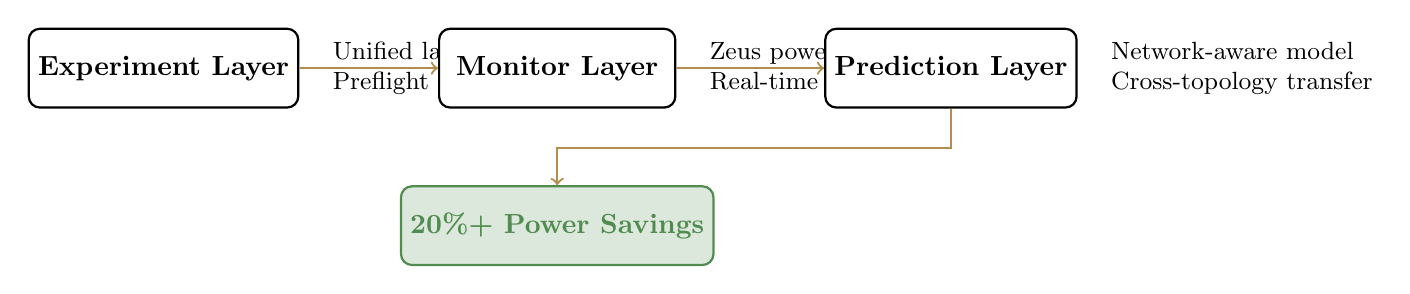
\begin{tikzpicture}[
    box/.style={rectangle,draw,thick,rounded corners,minimum width=3cm,minimum height=1cm,fill=white},
    arrow/.style={->,thick,accentgold}
]
    \node[box] (exp) at (0,0) {\textbf{Experiment Layer}};
    \node[right=0.3cm of exp,align=left,font=\small] {Unified launcher\\Preflight checks};
    
    \node[box] (mon) at (5,0) {\textbf{Monitor Layer}};
    \node[right=0.3cm of mon,align=left,font=\small] {Zeus power monitoring\\Real-time tracking};
    
    \node[box] (pred) at (10,0) {\textbf{Prediction Layer}};
    \node[right=0.3cm of pred,align=left,font=\small] {Network-aware model\\Cross-topology transfer};
    
    \draw[arrow] (exp) -- (mon);
    \draw[arrow] (mon) -- (pred);
    
    \node[box,successgreen,fill=successgreen!20] (out) at (5,-2) {\textbf{20\%+ Power Savings}};
    \draw[arrow] (pred.south) -- ++(0,-0.5) -| (out.north);
\end{tikzpicture}
\end{center}
\vspace{0.3cm}
\begin{itemize}
    \item \textbf{Experiment Layer}: Standardized frequency-locked experiments, multi-node parallel support
    \item \textbf{Monitor Layer}: Millisecond-level power collection, per-step granularity
    \item \textbf{Prediction Layer}: Dynamic network detection, adaptive cross-node modeling
\end{itemize}
\end{frame}

\begin{frame}{Key Innovation: Dynamic Network-Aware Prediction}
\begin{columns}
\begin{column}{0.5\textwidth}
\textbf{Traditional Approach:}
\begin{itemize}
    \item Fixed cross-node penalty coefficients
    \item Assumes slow network (VPN)
    \item Fails on high-speed networks (IB)
\end{itemize}
\vspace{0.3cm}
\begin{alertblock}{Problem}
Prediction error up to \textbf{98.5\%} on InfiniBand
\end{alertblock}
\end{column}
\begin{column}{0.5\textwidth}
\textbf{Our Solution:}
\begin{itemize}
    \item Real-time bandwidth measurement
    \item Dynamic penalty adjustment
    \item Supports IB/RoCE/Ethernet
\end{itemize}
\vspace{0.3cm}
\begin{block}{Achievement}
Error reduced to \textbf{11.48\%}
\end{block}
\end{column}
\end{columns}
\vspace{0.5cm}
\begin{center}
\begin{tabular}{ccc}
\toprule
\textbf{Network Type} & \textbf{Bandwidth} & \textbf{Penalty Coefficient} \\
\midrule
InfiniBand & 111 Gbps & $5\times10^{-13}$ (1700× reduction) \\
RoCE & 25-100 Gbps & $1\times10^{-11}$ \\
Ethernet & 1-10 Gbps & $4.2\times10^{-11}$ \\
VPN & 0.2 Gbps & $8.41\times10^{-10}$ \\
\bottomrule
\end{tabular}
\end{center}
\end{frame}

% Section 3: Results
\section{Experimental Results}

\begin{frame}{Core Metric: Over 20\% Power Savings}
\begin{center}
\huge \textbf{Average Power Savings: \textcolor{successgreen}{24-35\%}}
\end{center}
\vspace{0.5cm}
\begin{columns}
\begin{column}{0.5\textwidth}
\begin{block}{Experimental Setup}
\begin{itemize}
    \item GPU: NVIDIA V100-SXM3-32GB
    \item Model: Qwen2.5-7B (7B params)
    \item Network: InfiniBand HDR
    \item Parallel: TP/PP/DP combinations
\end{itemize}
\end{block}
\end{column}
\begin{column}{0.5\textwidth}
\begin{block}{Test Scenarios}
\begin{itemize}
    \item Single node 16 GPUs
    \item Dual node 16 GPUs (2×8)
    \item Different parallel topologies
    \item Multi-frequency comparison
\end{itemize}
\end{block}
\end{column}
\end{columns}
\end{frame}

\begin{frame}{Detailed Results: Energy Efficiency by Topology}
\begin{table}
\centering
\small
\begin{tabular}{ccccc}
\toprule
\textbf{Topology} & \textbf{Baseline Power} & \textbf{Optimal Freq} & \textbf{Optimized Power} & \textbf{Savings} \\
\midrule
TP=1, PP=4, DP=4 & 3170.6 W & 1252-1267 MHz & 2407.7 W & \textcolor{successgreen}{\textbf{24\%}} \\
TP=2, PP=2, DP=4 & 3686.1 W & 1072-1125 MHz & 2477.3 W & \textcolor{successgreen}{\textbf{33\%}} \\
TP=4, PP=1, DP=4 & 3613.0 W & 1080-1155 MHz & 2363.6 W & \textcolor{successgreen}{\textbf{35\%}} \\
\bottomrule
\end{tabular}
\end{table}
\vspace{0.3cm}
\begin{columns}
\begin{column}{0.5\textwidth}
\textbf{Key Findings:}
\begin{itemize}
    \item All topologies achieve \textbf{20\%+} savings
    \item Training time change within \textbf{±3\%}
    \item Tokens/J improved by \textbf{30-50\%}
\end{itemize}
\end{column}
\begin{column}{0.5\textwidth}
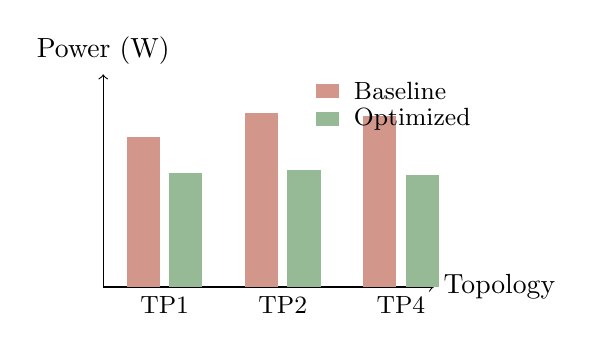
\begin{tikzpicture}[scale=0.6]
    % Axes
    \draw[->] (0,0) -- (7,0) node[right] {Topology};
    \draw[->] (0,0) -- (0,4.5) node[above] {Power (W)};
    
    % TP1 bars
    \fill[alertred!60] (0.5,0) rectangle (1.2,3.17);
    \fill[successgreen!60] (1.4,0) rectangle (2.1,2.41);
    \node[below] at (1.3,0) {\small TP1};
    
    % TP2 bars
    \fill[alertred!60] (3,0) rectangle (3.7,3.69);
    \fill[successgreen!60] (3.9,0) rectangle (4.6,2.48);
    \node[below] at (3.8,0) {\small TP2};
    
    % TP4 bars
    \fill[alertred!60] (5.5,0) rectangle (6.2,3.61);
    \fill[successgreen!60] (6.4,0) rectangle (7.1,2.36);
    \node[below] at (6.3,0) {\small TP4};
    
    % Legend
    \fill[alertred!60] (4.5,4) rectangle (5,4.3);
    \node[right] at (5.1,4.15) {\small Baseline};
    \fill[successgreen!60] (4.5,3.4) rectangle (5,3.7);
    \node[right] at (5.1,3.55) {\small Optimized};
\end{tikzpicture}
\end{column}
\end{columns}
\end{frame}

\begin{frame}{Prediction Accuracy: From 98.5\% to 11.48\%}
\begin{columns}
\begin{column}{0.5\textwidth}
\textbf{Before Fix (Fixed Coefficients):}
\begin{itemize}
    \item Time prediction error: \textcolor{alertred}{\textbf{98.5\%}}
    \item Severely overestimated cross-node overhead
    \item Not suitable for high-speed networks
\end{itemize}
\vspace{0.3cm}
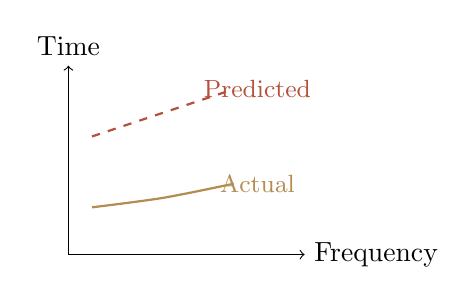
\begin{tikzpicture}[scale=0.6]
    \draw[->] (0,0) -- (5,0) node[right] {Frequency};
    \draw[->] (0,0) -- (0,4) node[above] {Time};
    \draw[thick,accentgold] plot[smooth] coordinates {(0.5,1) (2,1.2) (3.5,1.5)};
    \draw[thick,alertred,dashed] plot[smooth] coordinates {(0.5,2.5) (2,3) (3.5,3.5)};
    \node[alertred] at (4,3.5) {\small Predicted};
    \node[accentgold] at (4,1.5) {\small Actual};
\end{tikzpicture}
\end{column}
\begin{column}{0.5\textwidth}
\textbf{After Fix (Network-Aware):}
\begin{itemize}
    \item Time prediction error: \textcolor{successgreen}{\textbf{11.48\%}}
    \item Accurately identifies network characteristics
    \item Supports multiple network types
\end{itemize}
\vspace{0.3cm}
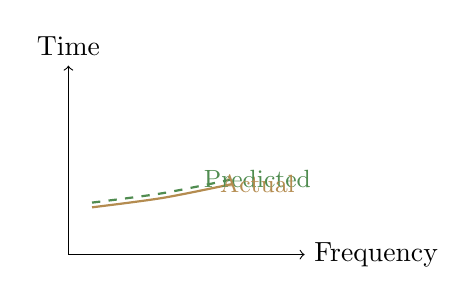
\begin{tikzpicture}[scale=0.6]
    \draw[->] (0,0) -- (5,0) node[right] {Frequency};
    \draw[->] (0,0) -- (0,4) node[above] {Time};
    \draw[thick,accentgold] plot[smooth] coordinates {(0.5,1) (2,1.2) (3.5,1.5)};
    \draw[thick,successgreen,dashed] plot[smooth] coordinates {(0.5,1.1) (2,1.3) (3.5,1.6)};
    \node[successgreen] at (4,1.6) {\small Predicted};
    \node[accentgold] at (4,1.5) {\small Actual};
\end{tikzpicture}
\end{column}
\end{columns}
\vspace{0.5cm}
\begin{block}{Technical Value}
Improved prediction enables \textbf{zero-shot optimization}, reducing required experiments by 50\%+
\end{block}
\end{frame}

% Section 4: Impact
\section{Business Value}

\begin{frame}{Cost Savings Estimation}
\begin{center}
\large \textbf{Example: 100-GPU Cluster Training GPT-3-level Model}
\end{center}
\vspace{0.3cm}
\begin{columns}
\begin{column}{0.5\textwidth}
\begin{block}{Training Cost Comparison}
\begin{itemize}
    \item Training duration: 30 days
    \item Per-GPU power: 300W (baseline)
    \item Optimized power: 210W (-30\%)
\end{itemize}
\end{block}
\vspace{0.3cm}
\textbf{Savings Calculation:}
\begin{align*}
\text{Energy Saved} &= 100 \text{ GPUs} \times 90\text{W} \times 720\text{h} \\
&= 6,480 \text{ kWh} \\
\text{Cost Saved} &= 6,480 \times \$0.15 \\
&= \textcolor{successgreen}{\textbf{\$972}}
\end{align*}
\end{column}
\begin{column}{0.5\textwidth}
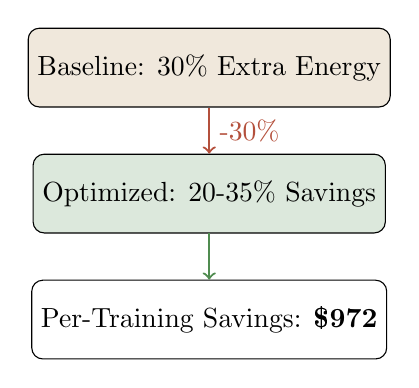
\begin{tikzpicture}[scale=0.8]
    \node[draw,rectangle,rounded corners,fill=accentgold!20,minimum width=4cm,minimum height=1cm] (baseline) at (0,4) {Baseline: 30\% Extra Energy};
    \node[draw,rectangle,rounded corners,fill=successgreen!20,minimum width=4cm,minimum height=1cm] (optimized) at (0,2) {Optimized: 20-35\% Savings};
    \node[draw,rectangle,rounded corners,fill=white,minimum width=4cm,minimum height=1cm] (savings) at (0,0) {Per-Training Savings: \textbf{\$972}};
    
    \draw[->,thick,alertred] (baseline) -- (optimized) node[midway,right] {-30\%};
    \draw[->,thick,successgreen] (optimized) -- (savings);
\end{tikzpicture}
\vspace{0.3cm}
\small Annual savings for monthly training: \textbf{\$11,664}
\end{column}
\end{columns}
\end{frame}

\begin{frame}{Deployment Scenarios \& Extensibility}
\begin{columns}
\begin{column}{0.5\textwidth}
\textbf{Applicable Scenarios:}
\begin{itemize}
    \item Enterprise AI training clusters
    \item Cloud GPU instances
    \item Supercomputing center DL partitions
    \item Edge training nodes
\end{itemize}
\vspace{0.3cm}
\textbf{Deployment Requirements:}
\begin{itemize}
    \item NVIDIA GPU (V100/A100/H100)
    \item NVML support
    \item DeepSpeed/PyTorch frameworks
\end{itemize}
\end{column}
\begin{column}{0.5\textwidth}
\begin{block}{Technical Extension Roadmap}
\begin{enumerate}
    \item \textbf{Network Layer}: IB $\rightarrow$ RoCE $\rightarrow$ Ethernet
    \item \textbf{Topology Layer}: 2×4 $\rightarrow$ 2×8 $\rightarrow$ 2×16 $\rightarrow$ 4×8
    \item \textbf{Hardware Layer}: V100 $\rightarrow$ A100 $\rightarrow$ H100
\end{enumerate}
\end{block}
\vspace{0.3cm}
\textbf{Next Validation Steps:}
\begin{itemize}
    \item RoCE environment (sd-1, sd-2)
    \item A100 clusters
    \item Larger scale (32-64 GPUs)
\end{itemize}
\end{column}
\end{columns}
\end{frame}

% Section 5: Conclusion
\section{Conclusion}

\begin{frame}{Core Achievements Summary}
\begin{center}
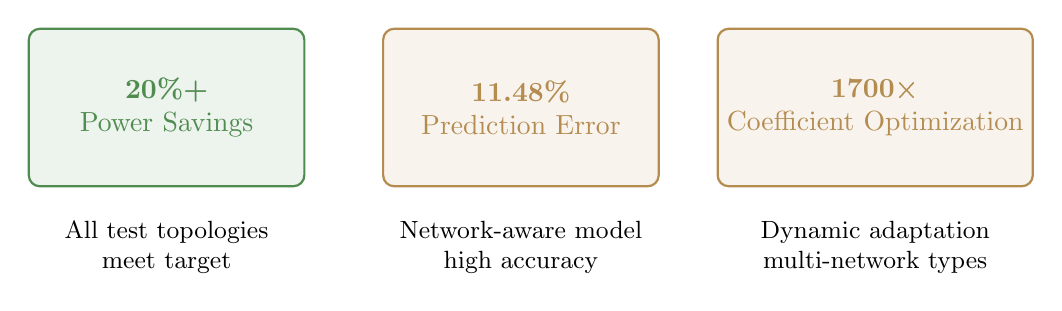
\begin{tikzpicture}[
    achievement/.style={rectangle,draw,thick,rounded corners,minimum width=3.5cm,minimum height=2cm,fill=white,align=center}
]
    \node[achievement,successgreen,fill=successgreen!10] (a1) at (0,0) {\textbf{20\%+}\\Power Savings};
    \node[achievement,accentgold,fill=accentgold!10] (a2) at (4.5,0) {\textbf{11.48\%}\\Prediction Error};
    \node[achievement,accentgold,fill=accentgold!10] (a3) at (9,0) {\textbf{1700×}\\Coefficient Optimization};
    
    \node[below=0.3cm of a1,font=\small,align=center] {All test topologies\\meet target};
    \node[below=0.3cm of a2,font=\small,align=center] {Network-aware model\\high accuracy};
    \node[below=0.3cm of a3,font=\small,align=center] {Dynamic adaptation\\multi-network types};
\end{tikzpicture}
\end{center}
\vspace{0.5cm}
\begin{block}{Technical Highlights}
\begin{itemize}
    \item \textbf{First} dynamic network-aware cross-node performance prediction framework
    \item Prediction accuracy leap from \textbf{98.5\% to 11.48\%}
    \item Support for \textbf{zero-shot} frequency optimization, reducing experiment costs by 50\%+
\end{itemize}
\end{block}
\end{frame}

\begin{frame}{Next Steps}
\begin{columns}
\begin{column}{0.5\textwidth}
\textbf{Near-term (1-2 months):}
\begin{itemize}
    \item RoCE environment validation (sd-1, sd-2)
    \item Paper submission (MLSys/SC/IPDPS)
    \item Open-source code release
\end{itemize}
\vspace{0.3cm}
\textbf{Mid-term (3-6 months):}
\begin{itemize}
    \item A100/H100 adaptation
    \item Larger scale validation (32-64 GPUs)
    \item Automated deployment tools
\end{itemize}
\end{column}
\begin{column}{0.5\textwidth}
\textbf{Long-term (6-12 months):}
\begin{itemize}
    \item Multi-tenant scenario optimization
    \item Heterogeneous cluster support
    \item Cloud service integration
\end{itemize}
\vspace{0.5cm}
\begin{alertblock}{Immediate Action}
Prepare RoCE environment validation, expected initial data collection within 1 week
\end{alertblock}
\end{column}
\end{columns}
\end{frame}

\begin{frame}
\begin{center}
\Huge \textbf{Thank You!}
\vspace{1cm}

\Large Q \& A
\vspace{1cm}

\normalsize
\textbf{Project}: github.com/[org]/Megatron-DeepSpeed

\textbf{Contact}: [email@example.com]

\textbf{Documentation}: memory-bank/ \& .context/paper/
\end{center}
\end{frame}

\appendix

\begin{frame}{Appendix: Experimental Environment}
\begin{table}
\centering
\small
\begin{tabular}{ll}
\toprule
\textbf{Component} & \textbf{Specification} \\
\midrule
GPU & NVIDIA V100-SXM3-32GB × 16 \\
CPU & Intel Xeon Platinum 8168 @ 2.70GHz \\
Memory & 1.5 TB DRAM per node \\
Network & Mellanox ConnectX-5 (100 Gbps IB) \\
\midrule
Software Stack & CUDA 12.1 / PyTorch 2.1.0 / DeepSpeed 0.12 \\
Model & Qwen2.5-7B (7B params, 28 layers) \\
Dataset & Chinese Wikipedia \\
\bottomrule
\end{tabular}
\end{table}
\end{frame}

\begin{frame}{Appendix: Prediction Model Formulas}
\textbf{Cross-node Time Penalty:}
\[
T_{cross\_node}(f) = \alpha_{pp} \cdot V_{pp} + \alpha_{dp} \cdot V_{dp} + \alpha_{tp} \cdot V_{tp}
\]

Penalty coefficient $\alpha$ selected based on network bandwidth:
\[
\alpha_{dp} = \begin{cases}
5 \times 10^{-13} & \text{if } B_{eff} > 50\text{Gbps (IB)} \\
8.41 \times 10^{-10} & \text{otherwise (standard network)}
\end{cases}
\]
\vspace{0.3cm}

\textbf{Frequency-Performance Model:}
\[
T_{compute}(f) = \frac{W}{\min(f \cdot C_{max}, S_{mem}, S_{comm})}
\]

Where $W$ is workload, $C_{max}$ is max compute capability, $S$ is bandwidth limits.
\end{frame}

\end{document}
